\chapter{Accurate Bike Routing}\label{ch:routing}

\begin{Summary}[Bibliographical Notes]
This chapter is based on the following paper in which the author was the principal investigator:

\cite{matthes2023accurate} \fullcite{matthes2023accurate}
\end{Summary}

\section{Introduction}

The mobility behavior in urban environments is becoming increasingly intermodal. The trend is moving towards a multimodal mobility planning \cite{park_framework_2023}, where bike-sharing and bike routes also play a significant role. Understanding cyclists' behaviors, particularly their route choices, is crucial not only for calculating preferences for suitable cycling routes but also as a fundamental aspect of expanding cycling infrastructure and urban planning \cite{zielstra_comparative_2011, huber_modelling_2021}. Models that replicate cyclists' route choices provide immediate insights into where cycling infrastructure should receive high priority. Thus, the application scenarios of bike routing are versatile and not strictly limited to navigation solutions.

To generate accurate routes for cyclists, one of the main challenges lies in the high individuality and context dependence of chosen paths \cite{dill_revisiting_2016, schleinitz_german_2017, misra_modeling_2018}, in which a multitude of criteria influence the optimal route \cite{song_exploring_2014}. Route choices depend not only on road conditions but also on factors such as bicycle type and personal preferences. Spontaneity also plays a role, ultimately leading to deviations from preselected routes that require appropriate rerouting.

In the context of GLOSA applications, routing is linked to additional factors. It is essential not only for the cycling route to follow reasonable paths but also to accurately align with bicycle lanes for precise traffic light matching. The closer the route aligns with the bicycle lane, the better it serves distance estimation to the traffic light. Accounting for bends or obstacles on the way to the traffic light ensures accurate distance estimation, preventing the speed recommendation from deviating from the actual speed. Additionally, factors such as route incline and road conditions contribute not only to routing but also serve as crucial information sources for speed recommendations. Accurate and consistent meta-information is desirable in these cases and can be obtained from an open or commercial routing foundation.

Commercial map providers provide highly accurate map material but have the drawback of limited openness and extensibility. Considerations about copyright, privacy, costs, and vendor lock-ins are also relevant for these map providers, rendering them unattractive for many services. Thus, various acknowledged routing apps resort to OpenStreetMap routing, such as Openrouteservice\footnote{\url{https://openrouteservice.org/}}, Photon and Komoot\footnote{\url{https://photon.komoot.io/}}, and Mapbox\footnote{\url{https://wiki.openstreetmap.org/wiki/Mapbox}}. Apple Maps and Bing Maps also use OpenStreetMap wherever no commercial data providers are available\footnote{\url{https://wiki.openstreetmap.org/wiki/Apple}, \url{https://wiki.openstreetmap.org/wiki/Bing_Maps}}. 

Despite being a highly recognized map foundation, an ongoing issue is that OpenStreetMap's accuracy and consistency vary due to its Volunteered Geographical Information (VGI) concept \cite{wasserman_evaluating_2019, jacobs_openstreetmap_2020, vybornova_automated_2023}. As a result, bicycle routes generated with OpenStreetMap may not always achieve the desired accuracy. With a highly engaged user base and various company-level contributors, OpenStreetMap profits from frequent updates. However, similar to Wikipedia, not all contributions are of high quality. As a result, bike paths are not always captured as separate geometries from the road or tagged with the correct properties.

In this chapter, we explore an alternative approach to enhance bicycle routing accuracy. Our proposal involves leveraging authoritative datasets, such as bike infrastructure reference models, that are maintained by institutions and distributed under open-source licenses. We focus our study on the "Digitales Radnetz Hamburg" (Digital Cycling Network Hamburg, DRN)\footnote{\url{https://metaver.de/trefferanzeige?docuuid=EA847D9F-6403-4B75-BCDB-73F831F960C7}}, a dedicated model for cycling paths in Hamburg. These models, including similar ones from other municipalities \cite{englede_efficient_2013, brovelli_towards_2017}, offer the potential for significantly improved precision and consistency in mapping cycling paths, making them a compelling solution for integration into a GLOSA app.

However, infrastructure reference models face the challenge of lacking global coverage. In the case of DRN, it covers only the city of Hamburg, making routing across city borders challenging. Solutions need to be devised for integrating the dataset with routing profiles for cyclists, addressing various technical challenges. Given that both DRN and OpenStreetMap lack elevation data, selecting the best provider from several available elevation providers is crucial. The goal is to outline precise steps that can help utilize similar datasets for bicycle routing in other regions and develop an open routing engine applicable beyond the GLOSA app for accurate bicycle routing in Hamburg.

Apart from the methodological aspect, the core contribution primarily lies in the results section. A key focus is evaluating how much the accuracy of traffic light matching can be improved with a potentially more precise representation of cycling paths, compared to results from \Cref{ch:matching}. The primary contribution is determining the effectiveness of routing based on this type of dataset by comparing alignment with the actual location of cycling infrastructure and the number of routing errors. The goal is to ascertain whether adopting the open DRN routing foundation can effectively address many of the issues encountered with OpenStreetMap bike routing, thereby providing users of the bike-GLOSA app with significantly improved directions and speed recommendations.

\section{Related Work}\label{sec:rw-uis}

Establishing an accurate bike routing is a multifaceted research area. One avenue of investigation focuses on models that can predict cyclists' route choices with high accuracy based on available metadata \cite{dill_understanding_2008, ghanayim_modelling_2018, huber_modelling_2021}. This involves correlating GNSS trajectories with routing networks to understand the relationships between path characteristics and route selection \cite{sultan_extracting_2017, huber_modelling_2021}. Some studies also focus on safe bike routing \cite{loidl_online_2018}, popularity-based routing \cite{bergman_conflation_2016} or the short-term effects of infrastructure changes on cyclists' route preferences \cite{yeboah_route_2015, pritchard_does_2019}. Over the years, open routing engines such as GraphHopper\footnote{\url{https://www.graphhopper.com/}} have continuously improved, providing community- and research-tested routing profiles tailored for various types of cycling. Thus, although there are optimization opportunities for bike routing profiles \cite{krismer_elevation_2016}, the available ones can be considered well consolidated.

Our focus will be on the issue of achieving a more accurate routing foundation and its application scenarios in GLOSA systems. First, we will discuss the status quo of bike path consistency and accuracy in routing foundations. Looking for solutions to the problem, we will investigate methods that utilize external authoritative datasets to improve the overall quality and alignment of bike path segments. Subsequently, we will delve into several challenges for GLOSA systems where precise routing emerges as a key solution.

\subsection{Bike Path Consistency and Accuracy in Routing Foundations}

How accurately and consistently a bike routing can be performed depends on the specific kind of routing foundation: VGIs such as OpenStreetMap, commercial providers such as Google Maps or Bing Maps, or authoritative infrastructure datasets.

Which routing foundation is best among multiple options is not a question that can be easily answered. Comparative research indicates that Google Maps and Bing Maps do not necessarily provide a more consistent and accurate depiction than OpenStreetMap. Ciepluch's investigation in 2010 \cite{ciepluch_comparison_2010} revealed that Google Maps, Bing Maps, and OpenStreetMap did not significantly differ in quality, with no platform emerging as a clear winner, while notable variations between cities could be identified.

The differences in mapping completeness between cities can be substantial. A recent study by Franzini et al. (2020) \cite{franzini_assessment_2020} found that only 40\% of the Pavia region in Italy is fully mapped in OpenStreetMap and 30\% in Google Maps, based on 2018 data. In other cities, the situation is considerably more favorable. Hochmair et al. (2015) \cite{hochmair_assessing_2015}, specifically assessing the coverage of bicycle infrastructure, found Portland to cover 86.4\% of 26 km of bicycle trails in OpenStreetMap and 78.4\% in Google Maps. This result stands in large contrast to the reported numbers for Miami, where only 22.8\% (OpenStreetMap) and 36.5\% (Google Maps) of 22 km of reference paths were accurately recorded, with a significant omission of paths along recreational sites such as rivers and parks. Thus, some cities require more substantial improvements to the mapping quality than others.

There also seem to be systematic issues that are not bound to specific cities. Ferster et al. (2019) \cite{ferster_using_2019} and Wasserman et al. (2019) \cite{wasserman_evaluating_2019} highlighted inconsistencies in meta-information about bike path quality in OpenStreetMap, impacting the determination of bikeability. Vybornova et al. (2023) \cite{vybornova_automated_2023} demonstrated that connectivity issues in bicycle path segments could disrupt meaningful route calculations. These disconnected bike path segments may arise from false editations to the map material.

In recent years, multiple solutions have been proposed that focus on flagging these issues for manual correction. In this course, authoritative datasets have been used as ground truths to identify issues, as demonstrated by various studies \cite{haklay_how_2010, jokar_arsanjani_quality_2015, ludwig_comparison_2011}. Brovelli et al. (2017) \cite{brovelli_towards_2017} introduced a framework for comparing open reference map data with OpenStreetMap, focusing on enhanced reusability. In their work, the authors propose specific metrics that can be utilized to identify city areas in which the mapping quality is exceptionally low.

Apart from flagging and quality-assurance helpers, there are also works that investigate automated error correction solutions. For example, Vybornova et al. (2023) \cite{vybornova_automated_2023} recently suggested a method to detect and rectify missing connections between bike paths. Nasiri et al. (2018) \cite{nasiri_improving_2018} introduced a multi-stage approach in which outliers are detected and removed from OpenStreetMap edit histories, improving the positional precision of features by 14\% in Teheran.  

Authoritative datasets have been investigated to fill in missing or inconsistent meta information for paths, by combining paths from the authoritative dataset to the OpenStreetMap network. Both Szwoch (2018) \cite{szwoch_combining_2019} and Fan et al. (2016) \cite{fan_polygon-based_2016} examine map-matching methods that have established themselves as a valuable tool to bridge topological differences between slightly offset map sources \cite{chao_survey_2020}. In a recent study, Meister et al. (2023) \cite{meister_route_2023} investigated cyclists' route choices in Zurich, using map-matching to incorporate metadata from a municipal dataset due to OpenStreetMap's insufficient consistency. The geometrical precision of OpenStreetMap bike path segments was not enhanced.

Two studies also employ a geometric modification to the path network. Smarzaro et al. (2021) \cite{smarzaro_creation_2021} investigated such an approach to reach a higher path coverage for multimodal routing. Their method involves comparing geospatial features from external datasets to nearby paths, adding new features if they don't overlap with existing ones. Li et al. (2017) \cite{li_optimized_2017} demonstrate the integration of OpenStreetMap into an authoritative bikeway dataset to primarily enhance coverage. Their semi-automated approach involves preprocessing datasets, an automatic conflation that maps metadata between formats, and human-in-the-loop adjustments for matching quality evaluation. 

Both studies convey promising methods, although no specific evaluation with ground truth, i.e., the actual position of bike paths, is presented. In general, more investigation is required to investigate the impacts of such a routing on general routing errors, alignment with bike paths, and the impacts of routing on traffic light matching as a crucial functionality for GLOSA applications.

\subsection{Routing in GLOSA Applications}

Building on the collected understanding of general challenges in routing, we will now focus on ongoing challenges in GLOSA applications that are directly or indirectly related to routing.

In a study by Sharara et al. (2019) \cite{sharara_impact_2019}, it has been shown that drivers need time to adapt to the speed advisory. One important factor for a timely speed advisory activation is detecting as early as possible during the ride which traffic light will be passed. As one possible solution, Mahler et al. (2012) \cite{mahler_reducing_2012} proposed using Google Maps to generate a route, selecting traffic lights even before the ride has started. As we have shown in \Cref{ch:matching}, most current approaches to select traffic lights are based on snapping the user location to the nearest traffic light geometry \cite{katsaros_performance_2011, bernais_design_2016, wilson_driver_2017, stahlmann_exploring_2018, bhattacharyya_assessing_2022}, not considering the predicted turns or general trajectory of the user. This leads to the issue that most current approaches delay the speed advisory's activation until a sufficient match can be determined. In some cases, the speed advisory may be hidden from the user even close to the traffic light due to a missing match \cite{wilson_driver_2017, stahlmann_exploring_2018}.

In our work (2022-2023) \cite{matthes2022matching, matthes2023geo}, we developed a matching procedure bringing the approach envisioned by Mahler et al. (2012) \cite{mahler_reducing_2012} into practice. Finding errors in the generated OpenStreetMap bike routes, the developed model was designed in a robust way, such that routing errors and inaccuracies were circumvented. Nonetheless, it was determined that attaining more accurate bike routes could benefit the described approach and provide a more accurate matching.

Another ongoing challenge is the practicality of multi-segment GLOSA. Proposed by Seredynski et al. (2013) \cite{seredynski_comparison_2013, seredynski_multi-segment_2013}, the idea of such systems is calculating an optimal speed for multiple consecutive traffic lights instead of only one, further decreasing the energy consumption of a vehicle. This method was further investigated by Xu et al. (2015) \cite{xu_bb_2015}, De Nunzio et al. (2015) \cite{de_nunzio_eco-driving_2015}, Nguyen et al. (2016) \cite{nguyen_efficient_2016}, and Simchon et al. (2020) \cite{simchon_real-time_2020}. In an analysis by Sharara et al. (2019) \cite{sharara_impact_2019}, a multi-segment GLOSA approach was found to be more robust against poor network performance. Nonetheless, at the moment, this idea has not been tested outside of simulations or controlled test beds. Predicting multiple consecutive intersections in a real environment is considered an ongoing challenge in GLOSA systems by Mellegård et al. (2020) \cite{mellegard_day_2020}. Performing accurate routing to more reliably select traffic lights in advance would represent one possible avenue for multi-segment approaches.

Strongly tied to accurate routing is also the task of distance-to-signal estimation. A precise estimate is required for all GLOSA applications that provide a direct speed advisory to the user. However, many studies neglect the opportunity to address this aspect in more detail, assuming that a straight-line distance between the user location and the traffic light is sufficiently accurate \cite{iglesias_i2v_2008, katsaros_performance_2011, koukoumidis_signalguru_2011, koukoumidis_leveraging_2012, krause_traffic_2012, li_open_2012, stevanovic_green_2013, stevanovic_comparative_2014, eckhoff_potentials_2013, gajananan_cooperative_2013, tal_vehicular-communications-based_2016, bernais_design_2016, stebbins_characterising_2017, sharara_impact_2019}. Only two studies suggest a different method for distance-to-signal estimation. In a study by Hao et al. (2019) \cite{hao_eco-approach_2019}, a map-matching algorithm is mentioned that positions the vehicle on its predefined trajectory along the test traffic lights. Xie et al. (2021) \cite{xie_dynamic_2021} utilize a predefined bus route to calculate the distance to the next intersection. These approaches could enhance the distance estimation in the presence of an accurate routing, also providing the potential to rectify the issue of GNSS inaccuracies.

Finally, another area for improvement in which routing plays a large role is context adaptivity. As discussed by Fickas et al. (2019) \cite{fickas_fast_2019}, cyclist applications demand a speed advisory to be given in a sensitive manner. Other studies by Tal et al. (2016) \cite{tal_vehicular-communications-based_2016} and Dabiri et al. (2020) \cite{dabiri_optimized_2020} conducted on cyclists investigate wind speeds as the main influencing factor for a speed advisory system. However, the bike path surface quality also plays a large role in bikeability \cite{wasserman_evaluating_2019} in addition to the path inclination, which has been studied as an influencing factor in studies on cars as well \cite{zhang_green_2020}. The necessary information could be acquired using a routing system, opening up new possibilities for a sensible speed advisory.

\begin{Summary}[Summary of Research Gap]
The main area for improvement in bike routing is the accuracy of bike maps. It is widely acknowledged that the depiction of bike paths in OpenStreetMap, but also in competitors such as Google Maps or Bing Maps, is often not ideal. Authoritative map material is often used as a ground truth to detect errors in the map foundations, but only a few studies investigate how authoritative maps could be utilized directly to improve a routing foundation's quality. Apart from utilizing map matching to gather more consistent metadata from the authoritative maps, two studies have focused on hybridizing VGIs with authoritative datasets, providing overall promising outlooks for the option to route on authoritative data. Instead of merging entire regions, these works have focused on merging individual paths. A more thorough investigation of the gainable accuracy relative to actual cycling infrastructure and intersection topologies is also required. Although there is a large variety of authoritative datasets, not all of these datasets may have a common format or quality, requiring a tailored solution.

Routing provides various new avenues for GLOSA research but has not been seen as an integral component thus far. Current approaches for traffic light matching lack consideration for predicted turns and user trajectory, resulting in delayed or even non-activation of speed advisories. Route-based approaches, seen as key enablers for multi-segment GLOSA systems, require more accurate bike routes to enhance traffic light matching accuracy. Distance-to-signal estimation is often oversimplified, with limited studies exploring alternatives to straight-line distance calculations. The potential of map-matching algorithms in addressing GNSS inaccuracies and improving distance estimation is also underexplored. Lastly, the context adaptivity of GLOSA systems for cyclists, considering factors like path surface quality and inclination, remains another area for improvement. Through delivering inclination and surface information, routing systems could play a pivotal role in acquiring necessary information for a more sensitive and tailored speed advisory, presenting an avenue for future research and development.
\end{Summary}

\section{Concept}

\subsection{DRN Routing}

Routing with GraphHopper and OpenStreetMap has the advantages of worldwide support and frequent updates of the community. However, the quality and consistency of the map materials vary from location to location. Since OpenStreetMap is a general-purpose map foundation, bike paths are often not represented as separate geometries but instead merged with the nearby road. This leads to the problem that some roads have separate bike path geometries running alongside, and others don't. Hence, when calculating a bike route based on OpenStreetMap, the bike route often jumps on or off the road. This degrades the distance-to-signal estimation, traffic light matching, and overall in-app routing. Although the system may work with OpenStreetMap, this situation is still not ideal.

To counteract this problem, it is vital to look for other routing foundations than OpenStreetMap that model the bike paths more accurately. As a solution, the dataset "Digitales Radverkehrsnetz Hamburg" (DRN) has been identified. The dataset is institutionally maintained and contains all bikeable paths in Hamburg. Based on preliminary comparisons with OpenStreetMap, the DRN dataset promises a more consistent and quality-assured depiction of bike paths.

\begin{figure}[htbp]
\centering
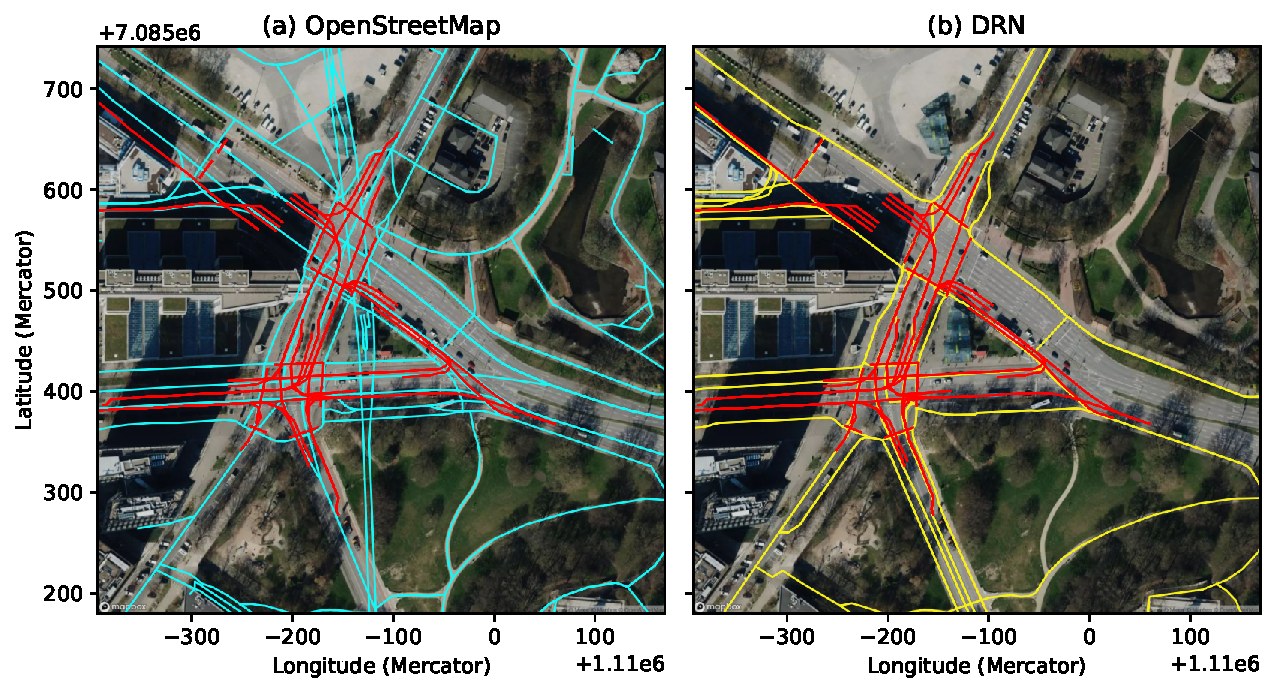
\includegraphics[width=\linewidth]{images/routing-drn-osm-intersection.pdf}
\caption{Alignment of OpenStreetMap vs. DRN with the intersection topology.}
\label{fig:comparison}
\end{figure}

\Cref{fig:comparison} shows a specific example of OpenStreetMap routing on the road when no separate bike path geometry is captured. With DRN the bike path is not only captured as a separate geometry but also aligns more closely with the bike path's curvature. Thus, the speed advisory could also be more precise as the signal's distance may be estimated more accurately. \Cref{fig:comparison} also highlights that the DRN route may align more closely with the bike signal's geometry, while the OpenStreetMap route is closer to the car lanes. Assuming that a cyclist follows the designated bike path, less speculation is required as to which traffic light must be matched. 

Due to these prospects, a system was created that allows for DRN-based bike routing inside Hamburg and OpenStreetMap-based bike routing outside Hamburg. To make DRN ready for routing, several processing steps were established as part of a publication at ITSC 2023 [in print], based on the supervised Diploma thesis of Max Lorenz (2022) \cite{lorenz_2022}: First, the DRN format must be translated into a data format that a routing engine understands. Then, the map's topology must be optimized such that routing errors are minimized. Finally, OpenStreetMap and DRN must be merged together at the city's border to allow a seamless transition.

\subsubsection{Translation from DRN to OpenStreetMap}

\begin{figure}[htbp]
\centering
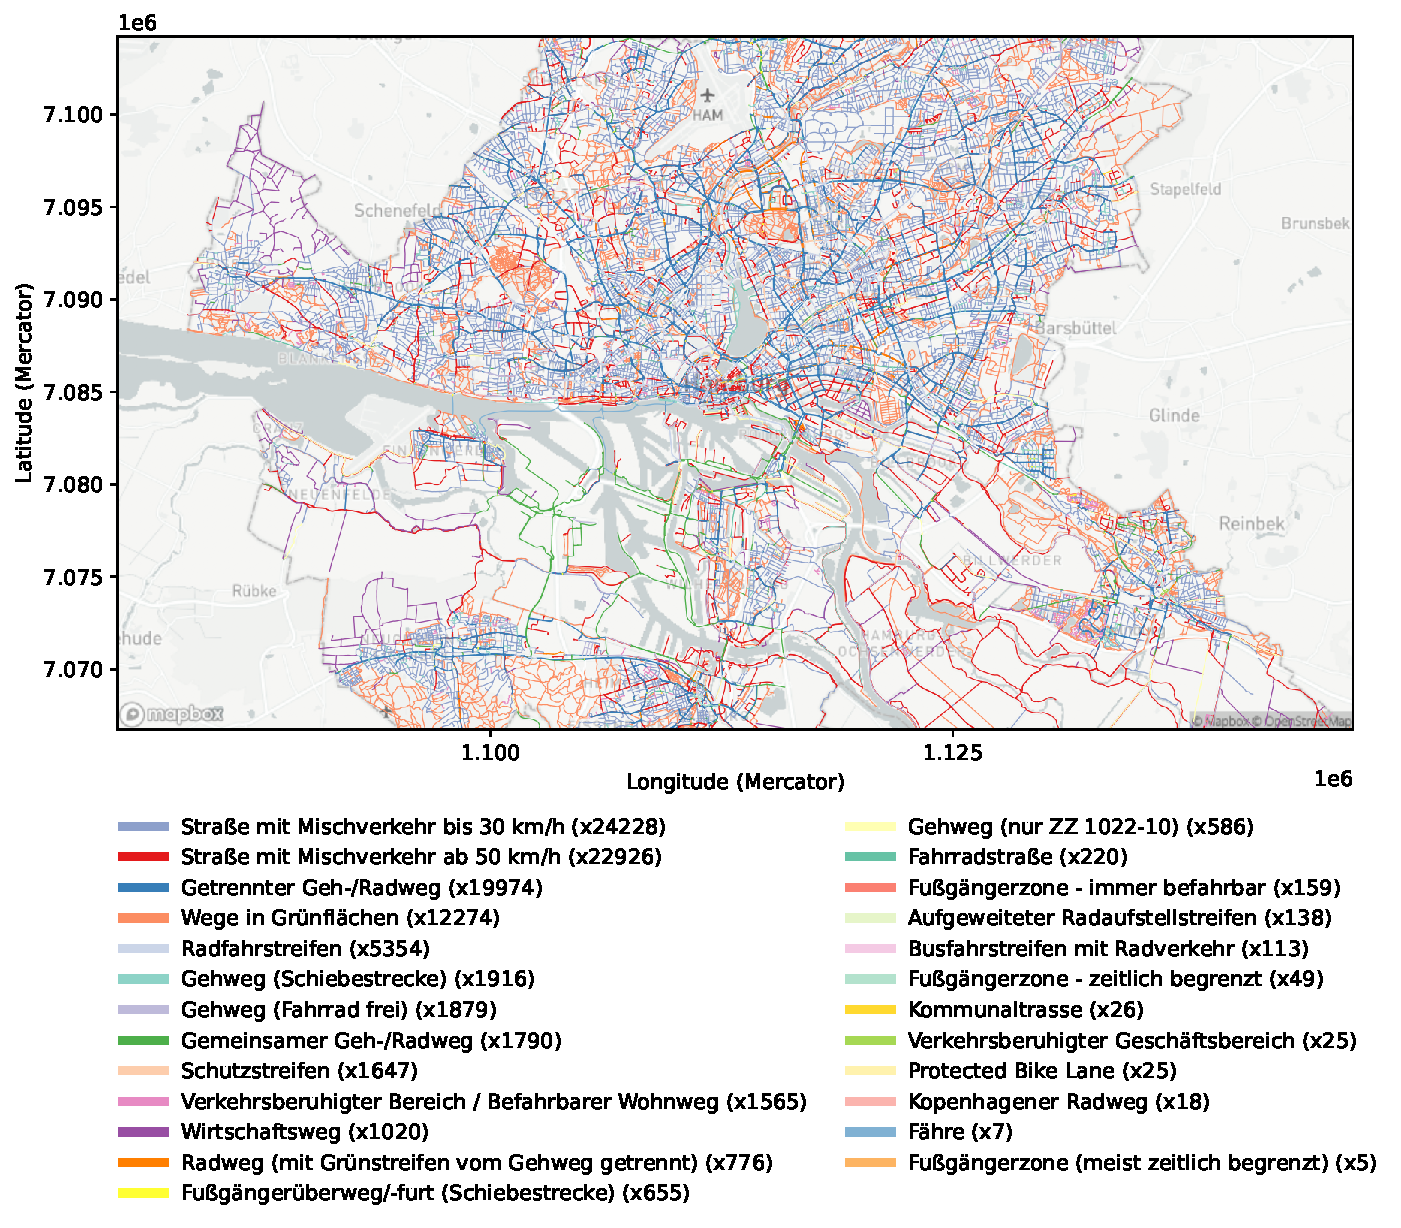
\includegraphics[width=\linewidth]{images/routing-drn.pdf}
\caption{An overview of the DRN dataset and its bike path types, as of Dec 23, 2023.}
\label{fig:drn-map}
\end{figure}

The DRN dataset can be downloaded in various geodata formats such as CSV, GeoJSON, or GML. Each contained data point refers to a path segment and is associated with metadata tags. Among others, the following properties are mapped\footnote{The displayed statistics represent a snapshot of the 23rd of August 2023.}:

\begin{itemize}
    \item Direction of travel (49852 segments bidirectional and 47692 segments unidirectional)
    \item Time restrictions (32 segments affected)
    \item Temporary paths such as pop-up lanes or detours (83 segments affected)
    \item If a segment is associated with a specific velo route or designated bike tours (Freizeitroute)
    \item Level (96237 flat, 1121 across bridges, 186 through tunnels)
    \item Obstacles (456 impassable, 52 can be circumvented e.g. via footpath)
    \item The type of bike path and its surface
    \item Target and end node ID of the segment connecting the segments to a graph
    \item The segment's coordinates
\end{itemize}

Now, to calculate routes based on the dataset, it is necessary to make the dataset available to the routing engine. Here, it is possible to design a plugin for the routing engine that allows it to read the dataset's format. However, a better solution is to transform the DRN dataset into the OpenStreetMap format. In this way, the existing routing engine and its community-tested routing profiles can be reused without modifying the engine's internals. Furthermore, transforming the DRN dataset to OpenStreetMap simplifies merging both datasets together at the city border. Thus, a map transformer was designed in [in print] that converts the DRN format to OpenStreetMap.

The routing profiles utilize weights of the properties annotated to each OpenStreetMap path to calculate a personalized route. The challenge here is that DRN specifies other properties than OpenStreetMap. For example, DRN specifies three types for compacted surface: "befestigt - nicht genauer erkennbar", "befestigt - zu detailieren" and "Wassergebundene Decke". To resolve this problem, a mapping was developed that infers the OpenStreetMap tags from the DRN specification. This mapping includes the bike path's surface, level, direction, and type (as shown in \Cref{fig:drn-map}). In cases where the bike path's properties cannot be directly mapped to a suitable OpenStreetMap tag, the path is tagged with \texttt{highway = tertiary}. As noted in [in print], this follows established mapping practices in Germany. The result is an inferred set of tags for each path in the OpenStreetMap format.

\subsubsection{Error Correction Methods}

After the map conversion into the OpenStreetMap format, there are still some problems with the map material that must be addressed. In [in print] two problems were identified when generating routes with the converted DRN network: detours resulting from duplicated nodes in the graph and detours because the road cannot be crossed.

\begin{figure}[htbp]
\centering
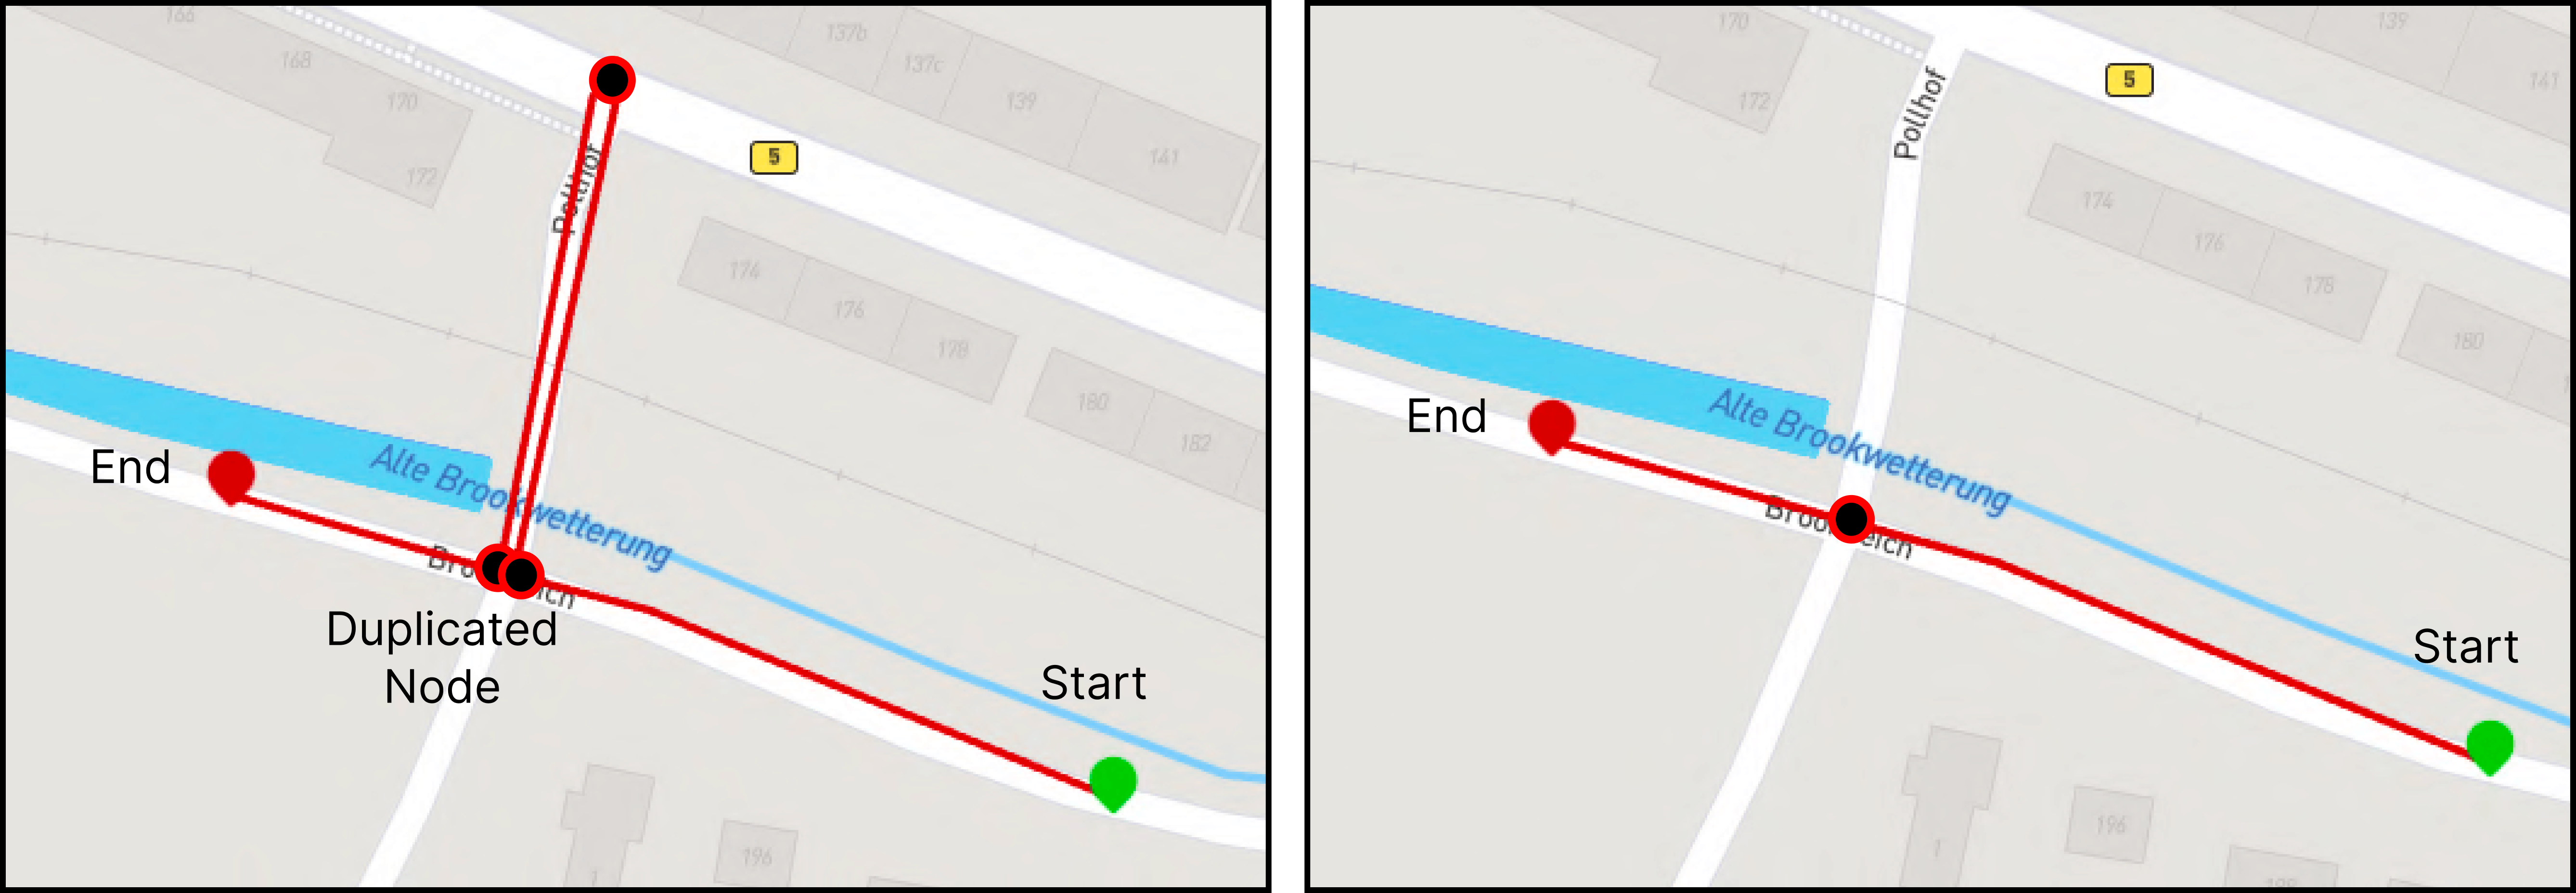
\includegraphics[width=\linewidth]{images/node-merging.png}
\caption{Duplicated nodes (left) are merged together (right) to avoid detours. Source: [in print]}
\label{fig:node-merging}
\end{figure}

\paragraph{Duplicated nodes:} Each individual path in the DRN dataset starts and ends in a node, which must be transformed into OpenStreetMap nodes that connect the individual paths to a graph structure\footnote{\url{https://wiki.openstreetmap.org/wiki/Node}}. To ease this process the DRN dataset provides node IDs for the start and end point of each path. Thus, two nodes are generated for each path based on the start and end coordinates given in the line geometry. Since there may be multiple paths that are connected to a node, the same node is generated multiple times during dataset processing. In theory, this is not a problem since the node ID can be utilized to avoid duplicates. In practice, however, sometimes there are nodes for which multiple different coordinates are found in the dataset. Due to presumably floating point or geographic projection inaccuracies in the dataset, the coordinates may be misaligned by a few centimeters.

As discussed in [in print], the developed solution involves calculating a center point for each node ID. Let $C_k = \{c_{k_1} = (lat_{k_1}, lng_{k_1}), \text{...} , c_{k_n} = (lat_{k_n}, lng_{k_n})\}$ be the collected coordinates for each node $k$. Then, the center point $\text{Center}_{\text{k}}$ is calculated as $\text{Center}_{\text{k}} = \left(n^{-1} * {\sum_{i=1}^{n} \text{{lat}}_{k_i}}, {n^{-1} * \sum_{i=1}^{n} \text{{lng}}_{k_i}}\right)$. The resulting coordinates are utilized to connect the generated paths. To validate this approach, the maximum relocation distance between all $\text{Center}_{\text{k}}$ and $c \in C_k$ was calculated as 8.3 centimeters using the haversine formula. Based on this result, no further points were falsely connected.

\paragraph{Non-crossable roads}: Since bike paths on both roadsides are captured as individual geometries in the DRN dataset, there may be long road segments with bike paths running in parallel. However, without interconnections between the roadsides, there is also no possibility for the route to cross the road. Sometimes, this represents a problem since side roads attached to the opposite roadside can only be reached by long detours. With OpenStreetMap, this is a lesser problem since roads are often captured as single-path geometries without a clear distinction between each roadside. 


\begin{figure}[htbp]
\centering
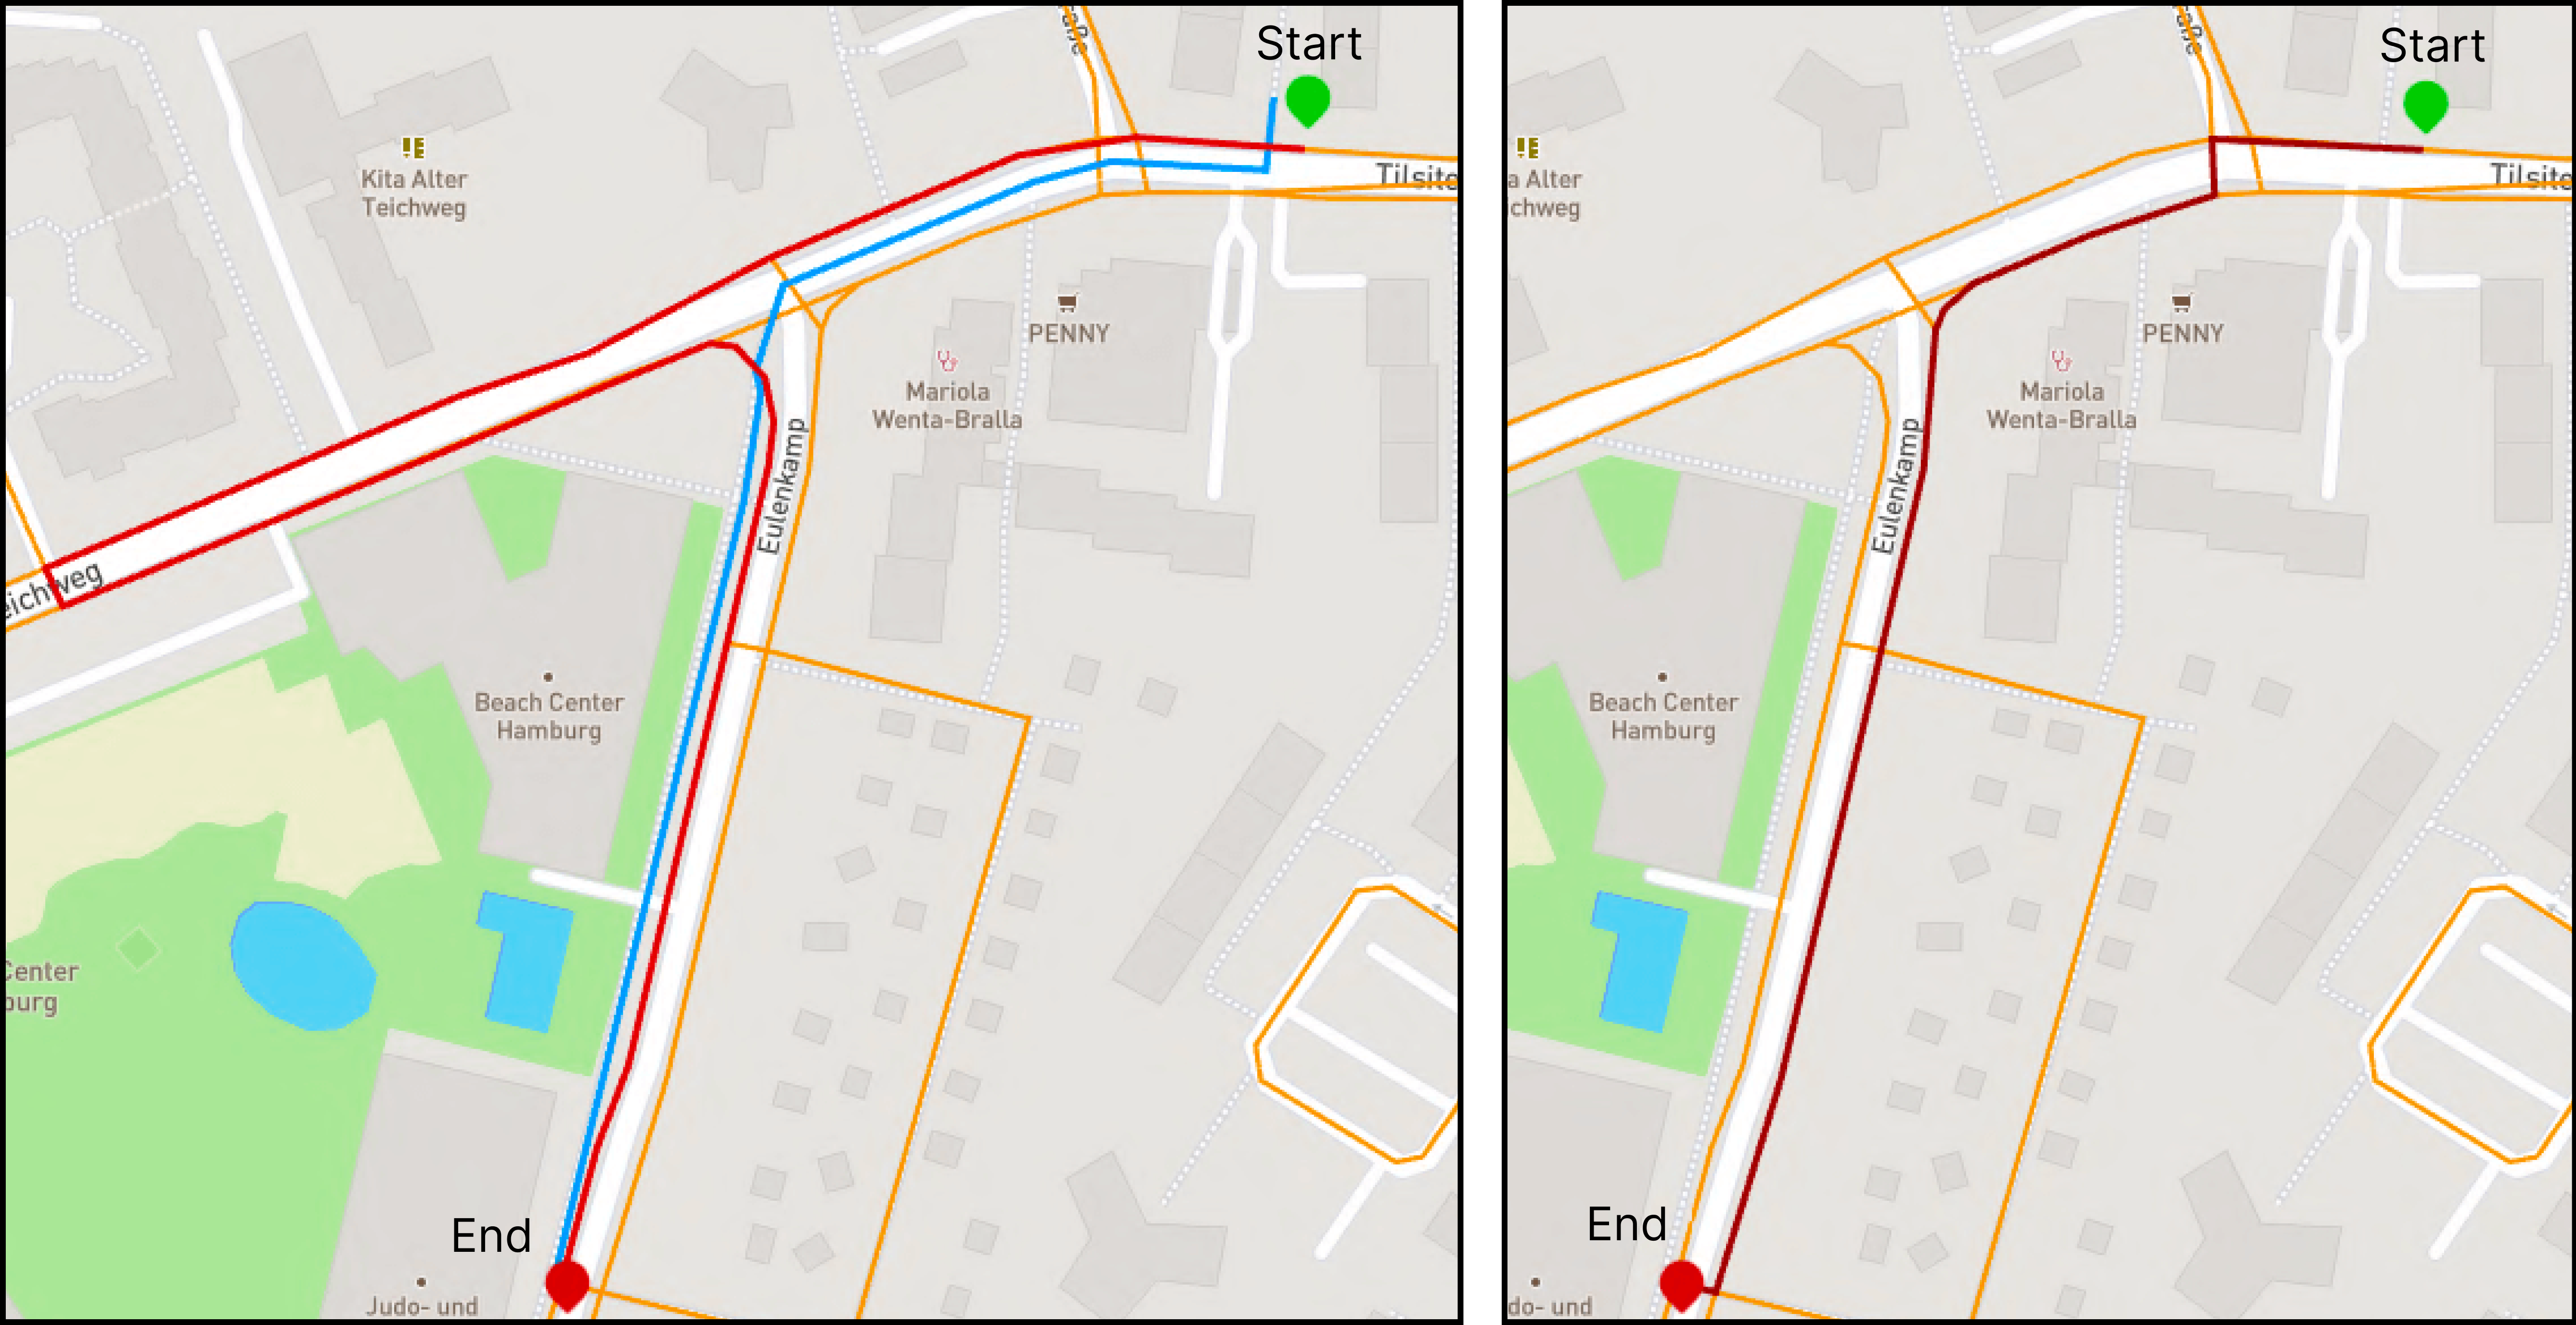
\includegraphics[width=\linewidth]{images/oneway-travel-fix.png}
\caption{Detour (left) that can be fixed by enabling opposite-direction one-way travel on foot (right), compared to OpenStreetMap route (blue). Source: [in print]}
\label{fig:oneway-travel-fix}
\end{figure}

One solution explored in [in print] is the introduction of "virtual" paths connecting the roadsides. Using these paths, the route could traverse between roadsides and avoid detours. Although this concept may sound like a reasonable idea at first, the question is where to place these virtual paths. For example, one could place these paths in a fixed interval along a road between roadsides. However, there could always be a physical barrier between both roadsides, meaning that generated routes would guide users over impassable obstacles or potentially encourage dangerous maneuvers. Traversing a road at an arbitrary location may not always be safe or legal. Due to these reasons, the idea of inserting virtual paths was discarded.

As discussed in [in print], the final solution takes another approach. In the DRN dataset, bike paths are marked for travel in one direction or two directions. Here, the error source for detours is often the restricted one-way travel direction along the bike path. In cases where detours are observed due to long paths down the street until the next road crossing, it is likely that a similar road crossing lies closer up the street. Thus, a solution is to allow opposite-direction one-way travel on foot. This solution assumes that the bike can safely and legally be dismounted and walked in the opposite direction.

\subsubsection{Routing Outside of Hamburg}

The DRN dataset's coverage ends at Hamburg's city border. This means that, although the dataset provides full coverage within the region of Hamburg, the dataset must be combined with another map foundation to provide routing outside the city. Here, it is possible to fall back to the OpenStreetMap dataset. However, the geometries of both datasets don't align. To provide continuous routing over the city border, both datasets must be stitched together. 

\begin{figure}[htbp]
\centering
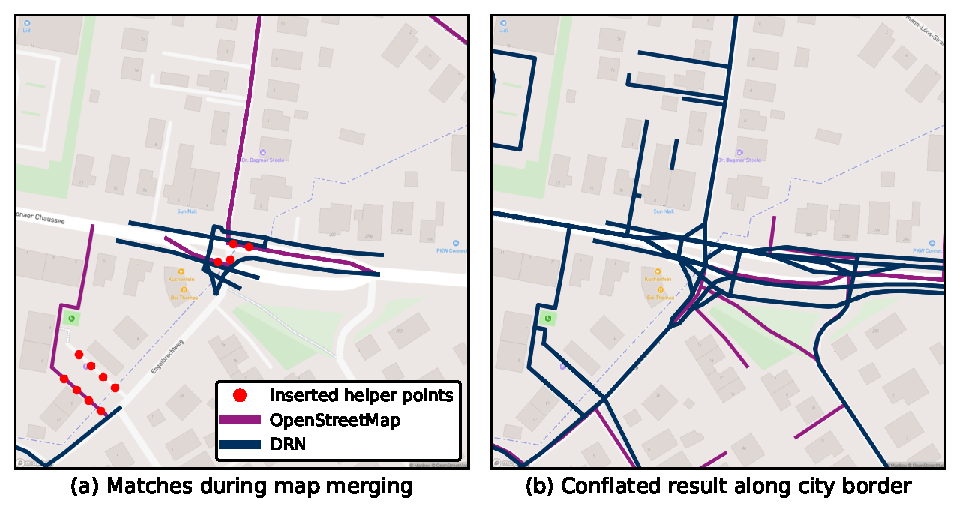
\includegraphics[width=\linewidth]{images/routing-drn-osm-border.pdf}
\caption{.}
\label{fig:}
\end{figure}

The conflation process presented in [in print] starts with matching the OpenStreetMap paths to the associated DRN paths along the city border. First, DRN nodes close (<20m) to the border are fetched. For each of these DRN nodes, the 5 nearest OpenStreetMap paths are treated as a possible match. However, the OpenStreetMap paths may traverse the city border without a node lying exactly on the border geometry, potentially leading to z-shaped connections between OpenStreetMap and DRN. To avoid this problem, the conflation process inserts artificial OpenStreetMap nodes at the intersection of the city border geometry. Finally, for each DRN node, the nearest (interpolated) OpenStreetMap node is selected and connected. As a result, the DRN paths are stitched to the OpenStreetMap paths along the city border.

Finally, the error-corrected and stitched path network is exported in the OpenStreetMap format. The exported map data is integrated with GraphHopper and replaces the original OpenStreetMap-only GraphHopper routing engine utilized by the mobile application.

\subsection{Digital Elevation Model}

With the chosen concept, users can personalize the routing algorithm to avoid inclines. In Hamburg, this may be less of a concern, but there are still several roads with non-negligible inclines such as Helgoländer Allee. However, DRN and OpenStreetMap don't directly include height data of the road network. Thus, without an external digital elevation model, the routing engine cannot consider paths accordingly using the specified routing profile. Fortunately, GraphHopper has a built-in option for integrating a digital elevation model.

As briefly discussed in [in print], there are multiple digital elevation models that can be used. By default, GraphHopper supports SRTM (Shuttle Radar Topography Mission) \cite{farr_shuttle_2000, farr_shuttle_2007} and CGIAR \cite{jarvis_hole_2008} height data. The CGIAR height data is a proprietary post-processed version of the SRTM data, filling in data gaps in the SRTM height map, and is available under license to all GraphHopper users. By default, the routing engine is specified to use the SRTM dataset.

SRTM-1 offers a horizontal resolution of approximately 30m (1 arcsecond). For specific areas, additional SRTM X-SAR 25m data is provided by the DLR. For the covered regions of the SRTM X-SAR 25m model, the vertical precision is specified at $\pm$ 6m (relative vertical error at 90\% confidence level)\footnote{SRTM X-SAR 25m specification: \url{https://geoservice.dlr.de/web/dataguide/srtm/}}. An even higher precision is offered by the DGM-1 model for Hamburg in which the 1 stands for 1 meter of horizontal resolution. In this model, the vertical resolution is specified as $\pm$ 15cm\footnote{\url{https://metaver.de/trefferanzeige?docuuid=A39B4E86-15E2-4BF7-BA82-66F9913D5640}}. The high precision is reached by airborne laser scanning. Downscaled resolutions are available as DGM-10 (10m) and DGM-25 (25m).

To evaluate if the DGM models provide an overall better height profile than SRTM, Max Lorenz analyzed cross-sections of the height models. Another important question of this work was how much resources the model consumes when loaded into the routing engine. The results, which have briefly been referenced in [in print], show that the best tradeoff between resource usage and model accuracy is provided by the DGM-10 model. Thus, the DGM-10 model was integrated as the final digital elevation model into the GraphHopper routing engine using a custom tileset download and parsing plugin. The result is a GraphHopper routing engine that not only runs on the DRN dataset but also utilizes the DGM-10 model to provide accurate, personalized routing while consuming an acceptable amount of resources. 

\subsection{Integration}

\paragraph{Distance-to-Signal Estimation:} In theory, the distance to the traffic light can be estimated directly along a straight line between the user and the signal. This may work if the speed advisory is enabled in proximity to the intersection, hereby assuming that the path to the traffic light is approximately straight. However, the goal is to enable the speed advisory as soon as possible, meaning that there may be multiple bends in the bike path until the user arrives at the signal. The linear distance alone is insufficient here as it underestimates the actual distance along the route curvature. 

Thus, it is crucial to incorporate map material into the estimation process. This represents a significant problem for speed advisory systems that have no understanding of the user's route. These systems have three options: choose the inherently inaccurate linear distance, employ a speculative map-matching algorithm for trajectory prediction, or calculate the distance along the provided intersection topologies. All of these approaches come with their own drawbacks that ultimately limit their accuracy with more distance from the intersection. However, these problems are not a concern here. The distance estimation is obtained by following the route, which captures the curved path of the bike infrastructure. This method assumes that the route closely aligns with the actual bike infrastructure, ensuring an accurate estimation.

\begin{figure}[htbp]
\centering
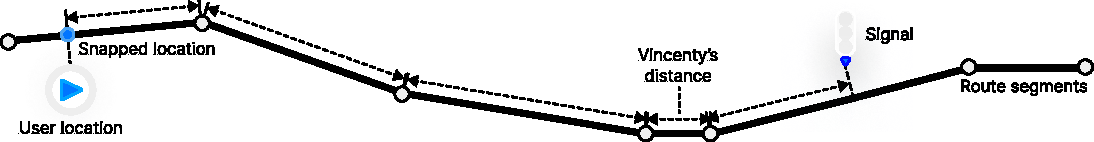
\includegraphics[width=\linewidth]{images/distance-to-signal-estimation.pdf}
\caption{Distance-to-signal estimation along the route curvature for speed recommendation.}
\label{fig:distance-to-signal-estimation}
\end{figure}

The specific process is highlighted in \Cref{fig:distance-to-signal-estimation}. First, the user's location is snapped to the route geometry, and the subsequent route segments are traversed until reaching the snapped location of the upcoming signal. Along these route segments, Vincenty's formulae are employed to precisely calculate the distance for each segment. Through precalculation of each segment's distance to the next signal, it is only necessary to calculate the distance along the current segment, and then add this segment's distance to the next signal. Therefore, this process is also very computationally efficient. The estimation process is repeated dynamically each time a new user location is received, updating the current speed advisory.

\paragraph{GNSS Error Correction:} Geolocation inaccuracies pose a significant concern for the designed app as they result in unintended movements of the map's camera tracking the user. In the worst-case scenario, the user's position may deviate completely from the intended route and enter nearby buildings. Tests conducted in Dresden indicate that older devices (Android 6) struggle more with GNSS drift than newer devices. However, even the latest generation of Android and iOS smartphones, configured to provide the highest level of geolocation accuracy, still experience this problem. \Cref{fig:battery-efficient-gps-error-correction} conceives two possible solution approaches.

\begin{figure}[htbp]
\centering
\resizebox{\linewidth}{!}{%
\begin{tabular}{p{0.5\linewidth}p{0.5\linewidth}}
  \multicolumn{1}{c}{\small{(a) Geolocation filtering.}} &
  \multicolumn{1}{c}{\small{(b) Error correction through route snapping.}} \\
  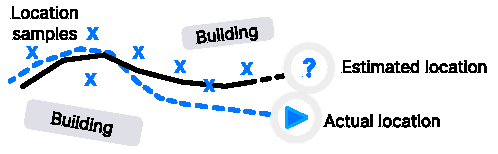
\includegraphics[width=\linewidth]{images/battery-efficient-gps-error-correction-1.pdf} &
  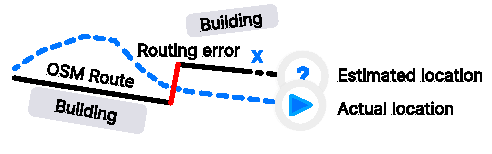
\includegraphics[width=\linewidth]{images/battery-efficient-gps-error-correction-2.pdf}  \\
\end{tabular}
}
\caption{Comparison of geolocation error correction approaches.}
\label{fig:battery-efficient-gps-error-correction}
\end{figure}

Filter-based error correction systems, such as Kalman filters, utilize the smartphone's inertial measurement unit (accelerometer, magnetometer, gyrosensor) to approximate the user's actual movement \cite{US20200049837A1}. These filters are useful in case no ground truth (the actual trajectory) is known but may imply an additional energy impact on the application. However, in the case of a bike-GLOSA application, the user will most likely have no energy source connected, which makes the energy impact a primary usability concern. Here, we can again take advantage of the user's generated route.

Assuming that the user strictly follows a predefined route, we can simply snap the user's location to the route, eliminating any GNSS scattering orthogonal to the route. Nonetheless, there are two notable issues with this approach. Firstly, there may be occasional errors in the route, requiring the routing to be as accurate to the bike path as possible. Secondly, geolocation scattering in the direction of the route is not eliminated. This effect can sometimes lead to problems at intersections. For instance, when approaching a traffic light slowly, the measured location may jump beyond the traffic light with respect to the route. 

To mitigate this problem, GNSS drift at an intersection is detected as follows: if the user is moving at a speed less than 2 meters per second, the app reverts to the last traffic light if it is within 10 meters of the user and no other traffic light is closer. This approach was tested through field tests in Hamburg and was perceived to be sufficient to compensate for the observed problem. However, in case a traffic light is still overshot, the user also has the option to manually select a traffic light by tapping on it in the map view.

\paragraph{Rerouting Strategy:} During a journey, users may occasionally deviate from the designated route. Since the app's speed recommendation relies heavily on the route, it is crucial to detect such deviations and recalculate the route dynamically. However, it is important to avoid triggering rerouting for minor GNSS errors when the user is still following the route accurately.

\begin{figure}[htbp]
\centering
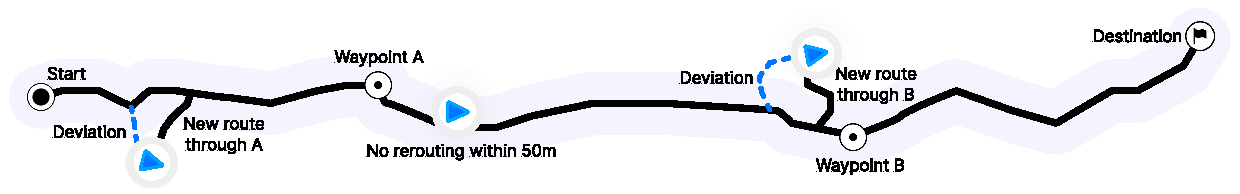
\includegraphics[width=\linewidth]{images/rerouting-strategy.pdf}
\caption{Schema of the rerouting procedure using a triggering threshold of 50 meters from the route.}
\label{fig:rerouting-strategy}
\end{figure}

The developed approach operates as follows: while the user is on the move, their location is continuously compared to the route by aligning it with the route geometry. The distance between the aligned location and the actual location is measured against a threshold. When the user moves significantly away from the route, exceeding the threshold, the rerouting is automatically initiated. A challenge in this approach is determining the appropriate distance threshold that strikes a balance between prompt rerouting and avoiding unnecessary recalculations. In initial tests conducted in Hamburg, a threshold of 20 meters was used. However, it proved to be too low and resulted in excessive unnecessary reroutings during field tests. Consequently, the threshold was increased to 50 meters, which yielded a satisfactory balance.

\begin{figure}[htbp]
\centering
\resizebox{\linewidth}{!}{%
\begin{tabular}{p{0.5\linewidth}p{0.5\linewidth}}
  \multicolumn{1}{c}{\small{(a) Rerouting via closest waypoint.}} &
  \multicolumn{1}{c}{\small{(b) Rerouting via virtual waypoint connection.}} \\
  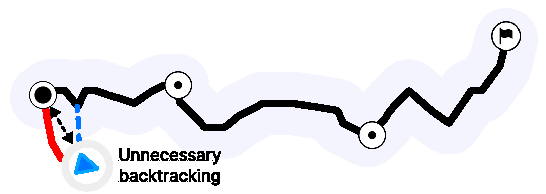
\includegraphics[width=\linewidth]{images/rerouting-strategy-1.pdf} &
  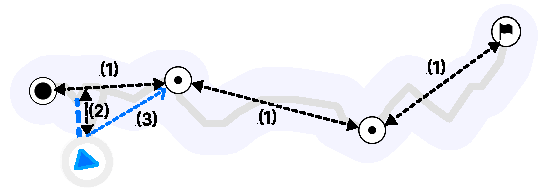
\includegraphics[width=\linewidth]{images/rerouting-strategy-2.pdf}  \\
\end{tabular}
}
\caption{Schematic comparison of the initial and final rerouting algorithms.}
\label{fig:rerouting-strategy-comparison}
\end{figure}

\paragraph{Selecting the Remaining Waypoints:} Another challenge in this approach is identifying the waypoints that have already been visited to prevent rerouting back to the starting point. To address this issue, only the remaining waypoints are selected when rerouting is triggered. Originally, the rerouting process involved selecting the nearest waypoint to the user and recalculating the route using that waypoint as a reference. However, this method was only effective half of the time, assuming the user's location was closer to the upcoming waypoint than to the previously visited waypoint. Consequently, this initial strategy often led to unnecessary backtracking.

Another option considered was snapping the user's location to the route geometry and following that path to find the next waypoint. However, a challenge arose because the waypoints were not directly integrated into the route geometry data structure, which is returned from the routing framework. Although it is possible to align the waypoints with the route geometry for implementation, a simpler and faster approximation was employed in the app, consisting of three steps: (1) Drawing direct lines between waypoints to create a connected path roughly resembling the route. (2) Selecting the nearest line to the user's location. (3) Determining the waypoint at the end of this line as the next waypoint for recalculating the route. This approach assumes that the drawn lines approximately represent the general route structure and has so far delivered quick and reliable rerouting during test rides.

\paragraph{Route Personalization:} Cyclist routes are highly individual and dependent on contextual circumstances. The problem is that there is a large variety of contextual factors, for example: elevation, grade of infrastructure separation, surface quality, traffic density, overall path length, speed limits, turn restrictions, or the number of traffic lights. The importance of these factors to the user may depend on additional factors such as personal habits, physique, bike type, or the type of activity (commute, sporting). As a result, providing the most suitable route can be stretched to an immensely complex modeling problem.

Modeling bike routes and incorporating user data into the process has established a research field in itself. However, it is important to focus on the goals of this work. After all, the ultimate goal is to develop a user-friendly overall concept for a bike-GLOSA app. It, therefore, makes more sense to first integrate an existing routing framework and then systematically identify points for improvement. Fortunately, through the continued efforts in the routing community, open-source routing engines have been developed that incorporate highly complex and field-tested routing profiles. The goal of this work is to leverage one of the publicly available routing engines and, if required, tune it to the needs of the bike-GLOSA app. For this work, the GraphHopper routing engine was selected preliminarily.

GraphHopper provides different \texttt{vehicle}s with individual path weights depending on the road's properties. Among these \texttt{vehicle}s are also various bike types such as \texttt{bike}, \texttt{bike2} (avoids inclines), \texttt{racingbike} or \texttt{mountainbike}. These profiles can be provided to the routing API to select a specific behavior, such as avoiding unpaved sections with the \texttt{racingbike} profile. The road network, together with metadata such as surface type, can be directly extracted from OpenStreetMap data. Since OpenStreetMap does not include height data, GraphHopper supports loading satellite-generated height maps. All in all, GraphHopper not only provides the option for personalized routing profiles but also for obtaining important metainformation about the route.

\begin{figure}[htbp]
\centering
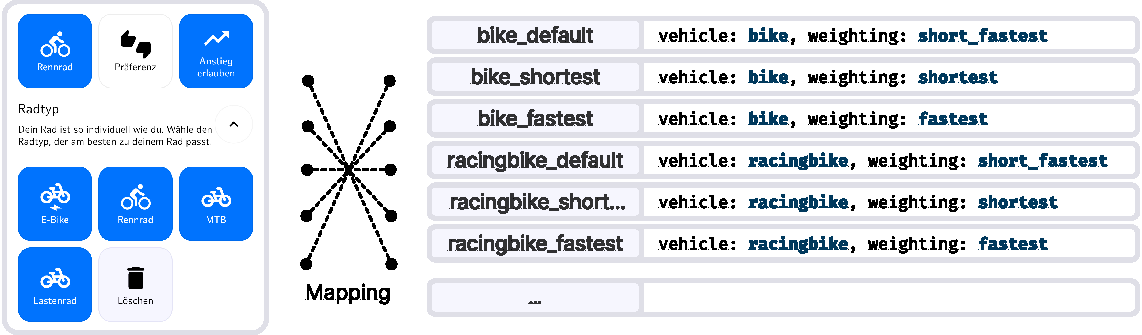
\includegraphics[width=\linewidth]{images/routing-profile-mapping.pdf}
\caption{Mapping of routing profiles for route personalization.}
\label{fig:routing-profile-mapping}
\end{figure}

The GraphHopper routing profiles are mapped to user-definable route preferences, as illustrated in \Cref{fig:routing-profile-mapping}. Three options are given to the user: bike type, general preference (short, fast route), and whether inclines should be avoided. Based on the user selection, a suitable routing profile is selected and utilized for calculating the routes. In case users don't specify a routing profile, a default routing profile (\texttt{bike2}) is selected that avoids inclines and utilizes the \texttt{short\_fastest} weighting, which represents a compromise between the short and fast weightings.

\paragraph{Updating the Map Materials:} The routing data must dynamically adapt to changes in the real world. With OpenStreetMap, the advantage is that the underlying road network is continuously updated by the community. Other open datasets have defined update intervals, such as the construction site dataset, which is updated every seven days\footnote{\url{https://metaver.de/trefferanzeige?docuuid=7A3772AB-3044-4D8D-9A0E-3DC03DF0EA3D}}. To provide up-to-date routing and map overlays, the respective backend services must be updated and associated data reprocessed. 

\begin{figure}[htbp]
\centering
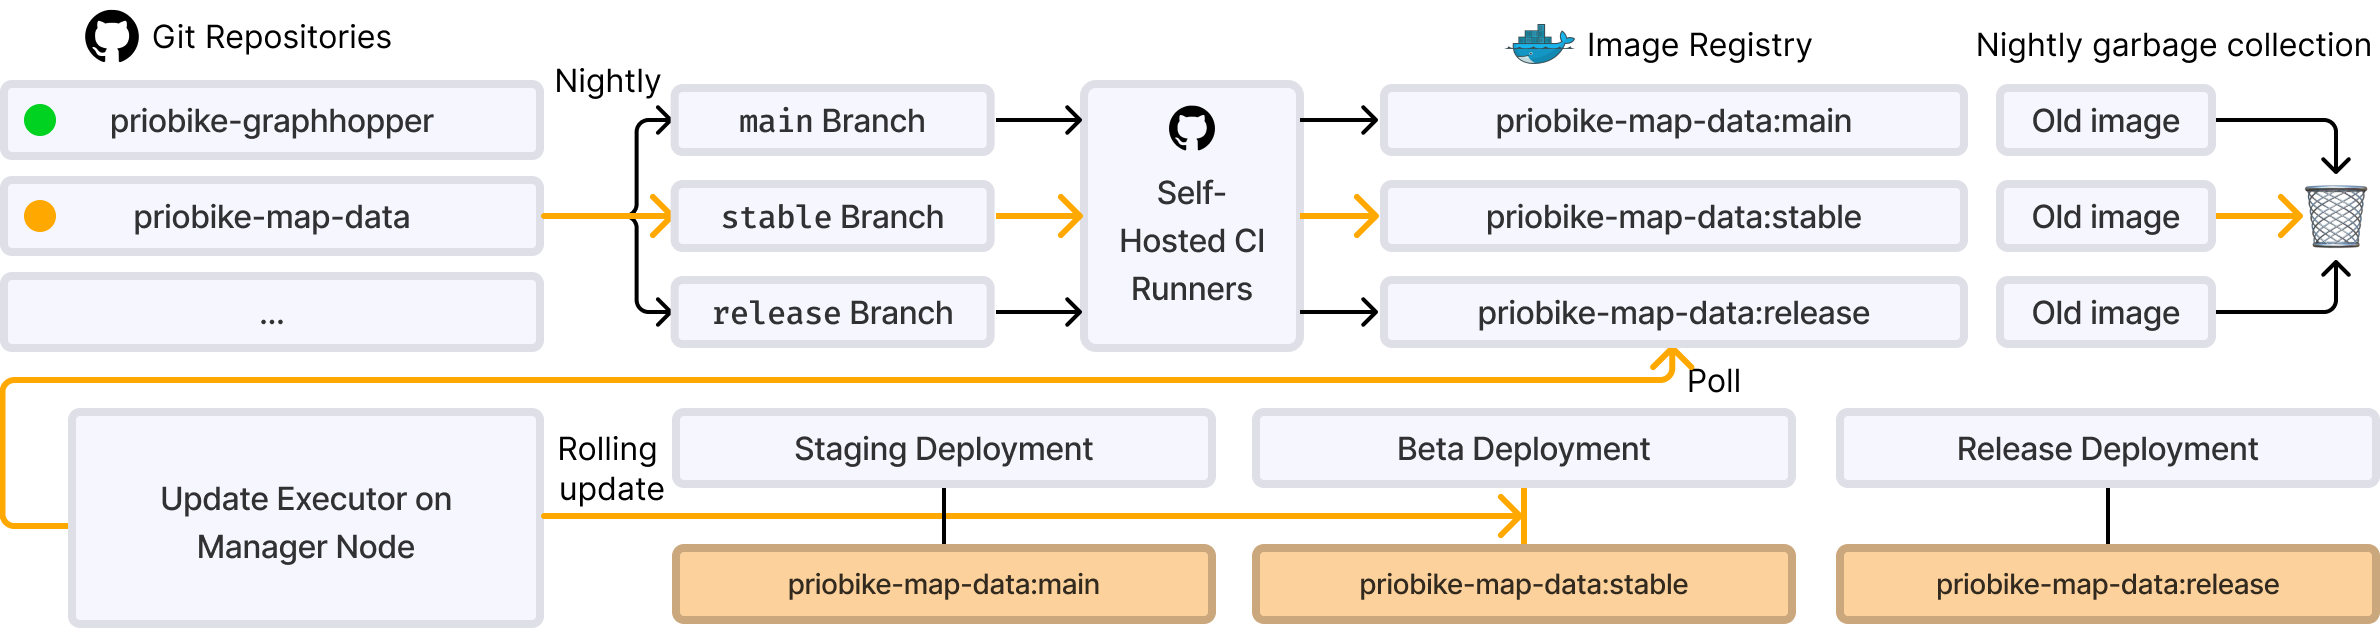
\includegraphics[width=\linewidth]{images/multi-stage-continuous-deployment.png}
\caption{Automated update pipeline for deployment services.}
\label{fig:multi-stage-continuous-deployment}
\end{figure}

To automate the update process, a CI/CD pipeline is utilized. The pipeline is highlighted in \Cref{fig:multi-stage-continuous-deployment}. Through a nightly build, new map data is fetched and processed. The final data is persisted in a Docker image and stored in a Docker registry. An update executor on the deployment VM notices the updated Docker image and replaces the currently deployed service, ensuring that the running services work with the newest map materials.

\section{Results}

\begin{figure}[htbp]
\centering
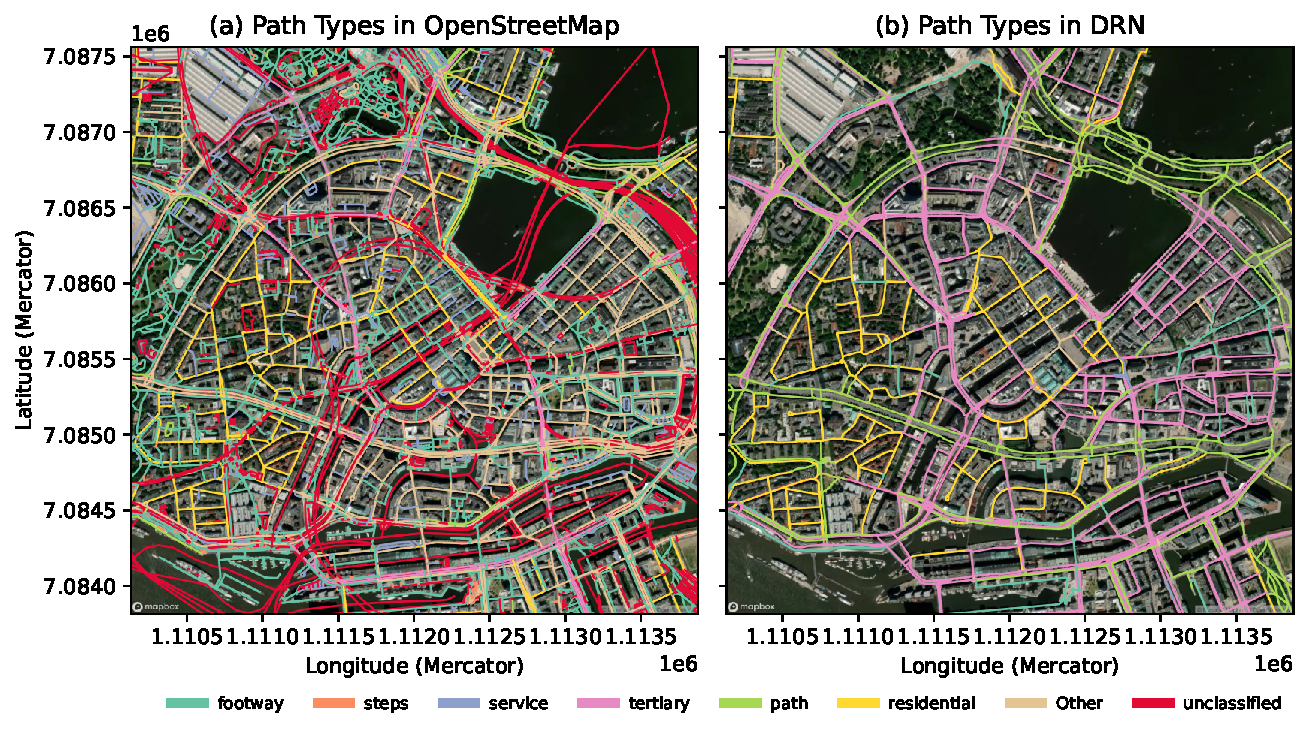
\includegraphics[width=\linewidth]{images/routing-drn-osm-map.pdf}
\caption{Mapping of metadata tags.}
\label{fig:}
\end{figure}

\subsection{Alignment with Actual Cycling Infrastructure}

\begin{figure}[htbp]
\centering 
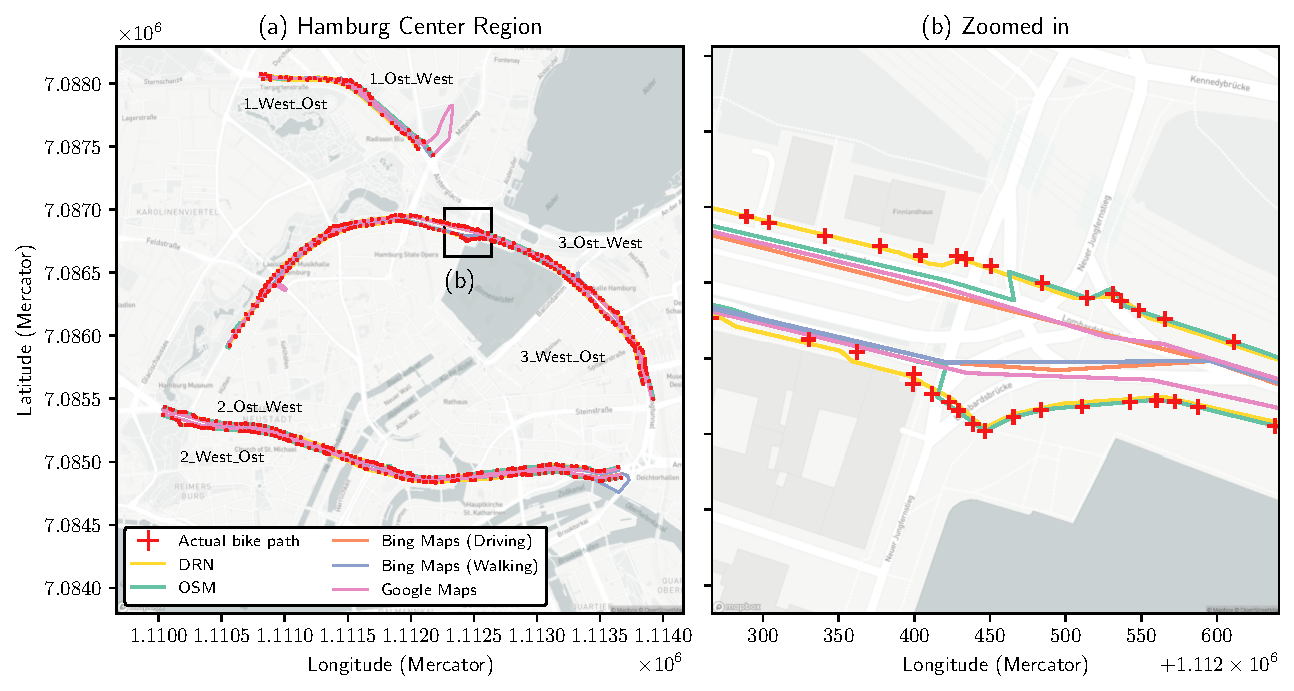
\includegraphics[width=\linewidth]{images/routing-hand-drawn-ground-truth.pdf}
\caption{.}
\label{fig:}
\end{figure}

\begin{table}[htbp]
\centering
\begin{tabular}{cccccc}
\hline
Hand-Drawn & Nr. of &\multicolumn{2}{c}{Cycling Network} & \multicolumn{2}{c}{OSM} \\
Reference Track & Signals & Hausdorff & Mean & Hausdorff & Mean \\ \hline
1 East-West ({1.0}{km}) & 4 & {6.89}{m} & {2.28}{m} & {10.52}{m} & {2.38}{m} \\
1 West-East ({1.2}{km}) & 6 &{2.80}{m} & {1.29}{m} & {9.10}{m} & {5.78}{m} \\
2 East-West ({2.2}{km}) & 12 & {3.49}{m} & {0.88}{m} & {18.22}{m} & {7.43}{m} \\
2 West-East ({2.6}{km}) & 12 & {3.67}{m} & {0.95}{m} & {24.07}{m}  & {10.00}{m} \\
3 East-West ({2.7}{km}) & 14 & {5.13}{m} & {0.91}{m} & {17.56}{m} & {8.00}{m} \\
3 West-East ({2.5}{km}) & 10 & {5.39}{m} & {1.70}{m} & {24.45}{m} & {8.35}{m} \\ \hline
\end{tabular}
\caption{Measured deviations from actual bike infrastructure.}%
\label{tab:accuracy-comparison}%
\end{table}

\begin{table}[htbp]
\centering
\begin{tabular}{lcc}
\hline
\textbf{Observed Error Cases} \\ \hline
Continuous routing on the road & 0 & 10 \\
Routing through buildings or stairs & 0 & 2 \\
Intersection crossing using car lanes & 0 & 8 \\
Use of sidewalks on incorrect road side & 1 & 4 \\
Missing permission for one-way streets & 0 & 1 \\
Routing through other impassable obstacles & 0 & 2 \\
Failure to consider turning restrictions & 0 & 1 \\
Skipping or crossing additional signals & 1 & 3 \\
Generally problematic road crossings & 1 & 4 \\
\hline
\end{tabular}
\caption{Observed error cases among arbitrary sample of 72 routes.}%
\label{tab:accuracy-comparison}%
\end{table}

\subsection{Influence on Traffic Light Matching}

\begin{figure}[htbp]
\centering 
\begin{tabular}{ccc}
\footnotesize{(b) OSM 2023} & \footnotesize{(b) DRN 2023}  \\
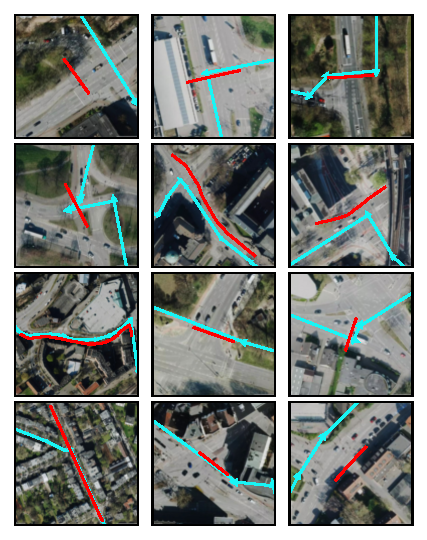
\includegraphics[width=0.46\linewidth]{images/routing-lane-alignment-examples-osm.pdf} & 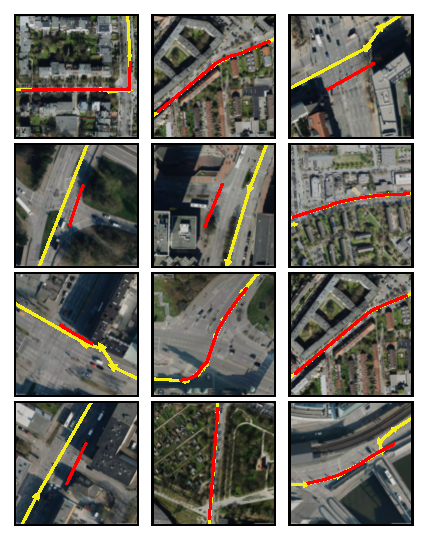
\includegraphics[width=0.46\linewidth]{images/routing-lane-alignment-examples-drn.pdf} \\
\end{tabular}
\caption{.}
\label{fig:}
\end{figure}

\begin{figure}[htbp]
\centering 
\begin{tabular}{cc}
\footnotesize{(a) Redundancy in OSM Ground Truth (2023)} & \footnotesize{(b) Redundancy in DRN Ground Truth (2023)} \\
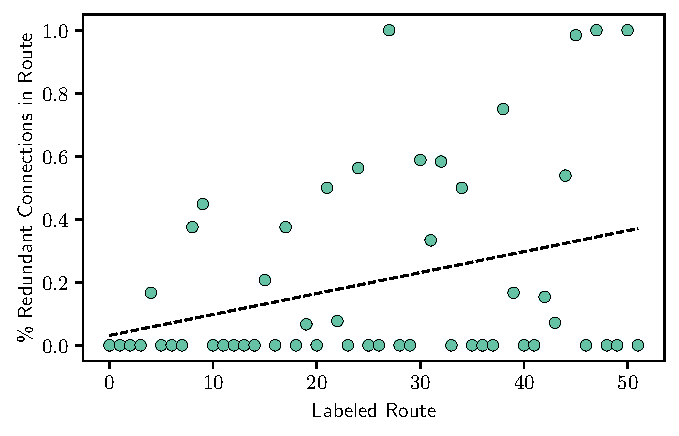
\includegraphics[width=0.45\linewidth]{images/matching-ground-truth-progression-osm.pdf} & 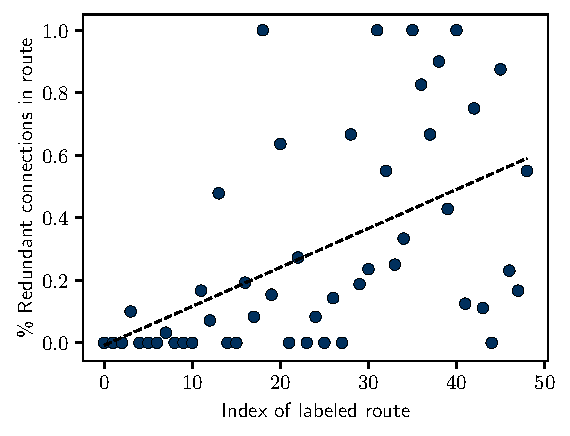
\includegraphics[width=0.45\linewidth]{images/matching-ground-truth-progression-drn.pdf} \\
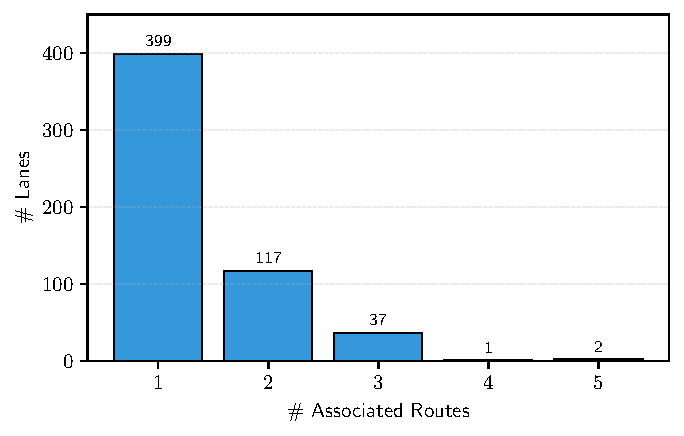
\includegraphics[width=0.45\linewidth]{images/matching-ground-truth-lsas-per-route-osm.pdf} & 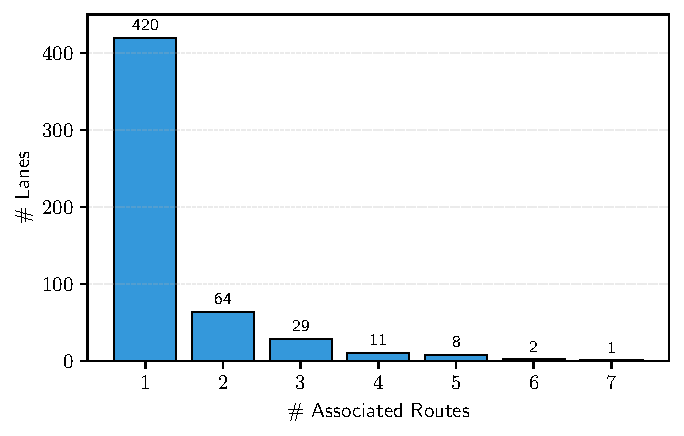
\includegraphics[width=0.45\linewidth]{images/matching-ground-truth-lsas-per-route-drn.pdf} \\
\end{tabular}
\caption{.}
\label{fig:}
\end{figure}

\begin{figure}[htbp]
\centering 
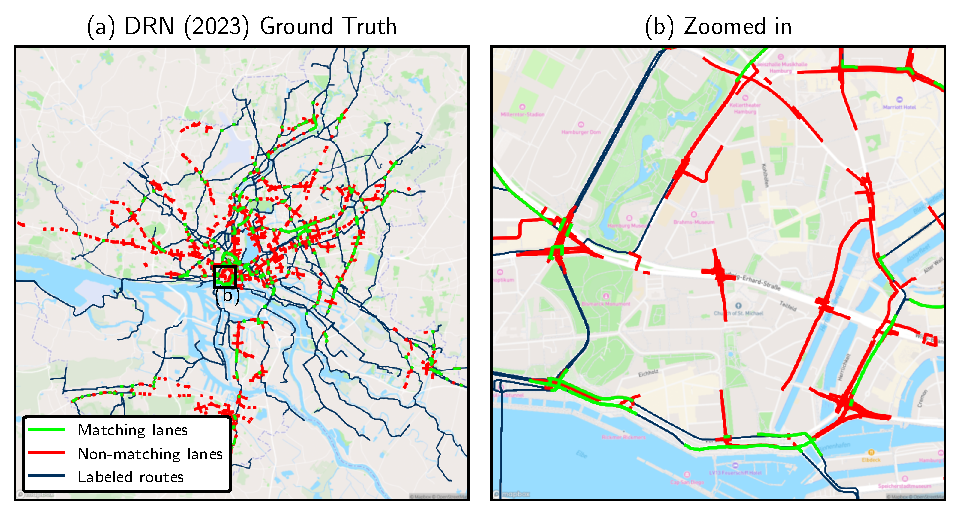
\includegraphics[width=\linewidth]{images/matching-ground-truth-drn.pdf}
\caption{.}
\label{fig:}
\end{figure}

\begin{table}[h]
\caption{Retrained model thresholds on the new routing.}
\begin{tabular}{@{}llllllllll@{}}
\toprule
  \textbf{Ground Truth} & $t_{dist}$ & $t_{bear}$ & $t_{bear\_sum}$ & $t_{inv}$ & $t_{len}$ & $t_{len\_sum}$ & $t_{road\_side}$ &  $t_{perfect\_m.}$ & $t_{overlap}$ \\
  \midrule
  OSM (2022) & 20m & 33° & 79\% & False & 0.99 & 93\% & 59m & 50m & 43\% \\
  OSM (2023) & 19m & 50° & 78\% & False & 0.96 & 77\% & 95m & 46m & 5\% \\
  DRN (2023) & 17m & 27° & 73\% & False & 0.81 & 61\% & 48m & 43m & 59\% \\
\bottomrule
\end{tabular}
\label{tab:hyperparameter-tuning-results-drn}
\end{table}

\begin{table}[h]
\caption{.}
\begin{tabular}{@{}lllllllll@{}}
\toprule
  \textbf{Model} & \textbf{Benchmark} & \textbf{Trained on} & \textbf{TP} & \textbf{FP} & \textbf{FN} & \textbf{Precision} & \textbf{Recall} & \textbf{F1} \\
  \midrule
  Algorithmic & OSM 2022 & OSM 2022 & 920 & 207 & 123 & 82\% & 88\% & 84.8\% \\
  Algorithmic & OSM 2022 & OSM 2023 & 908 & 221 & 135 & 80\% & 87\% & 83.6\% \\
  ML          & OSM 2022 & OSM 2022 & 936 & 57 & 107 & 94\% & 90\% & 91.9\% \\
  \midrule
  Algorithmic & OSM 2023 & OSM 2022 & 615 & 159 & 143 & 79\% & 81\% & 80.3\% \\
  Algorithmic & OSM 2023 & OSM 2023 & 637 & 136 & 121 & 82\% & 84\% & 83.2\% \\
  ML          & OSM 2023 & OSM 2022 & 614 & 52 & 144 & 92\% & 81\% & 86.2\% \\
  \midrule
  Algorithmic & DRN 2023 & DRN 2023 & 655 & 95 & 83 & 87\% & 89\% & 88.0\% \\
  ML          & DRN 2023 & DRN 2023 & 676 & 24 & 62 & 97\% & 92\% & 94.0\% \\
\bottomrule
\end{tabular}
\label{tab:model-scores-drn}
\end{table}

\begin{figure}[htbp]
\centering 
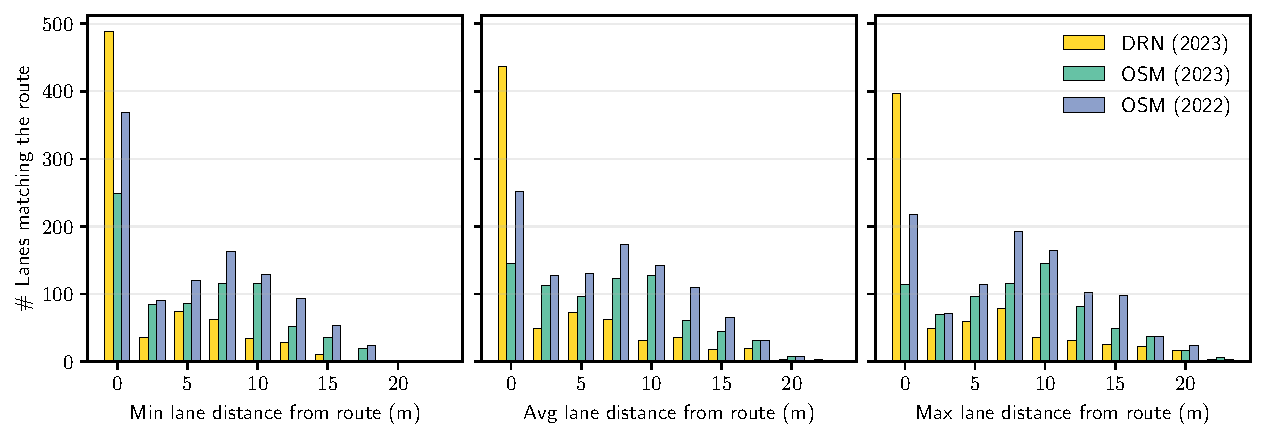
\includegraphics[width=\linewidth]{images/routing-lane-alignment.pdf}
\caption{.}
\label{fig:}
\end{figure}

\begin{figure}[htbp]
\centering 
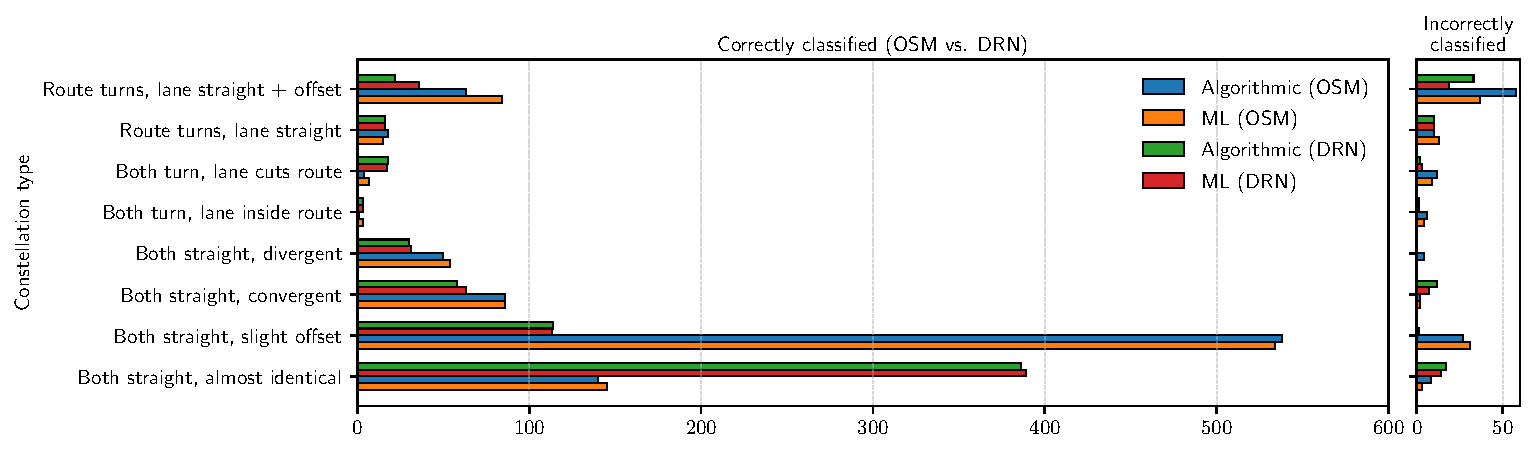
\includegraphics[width=\linewidth]{images/matching-constellations-osm-vs-drn.pdf}
\caption{.}
\label{fig:}
\end{figure}

\begin{figure}[htbp]
\centering 
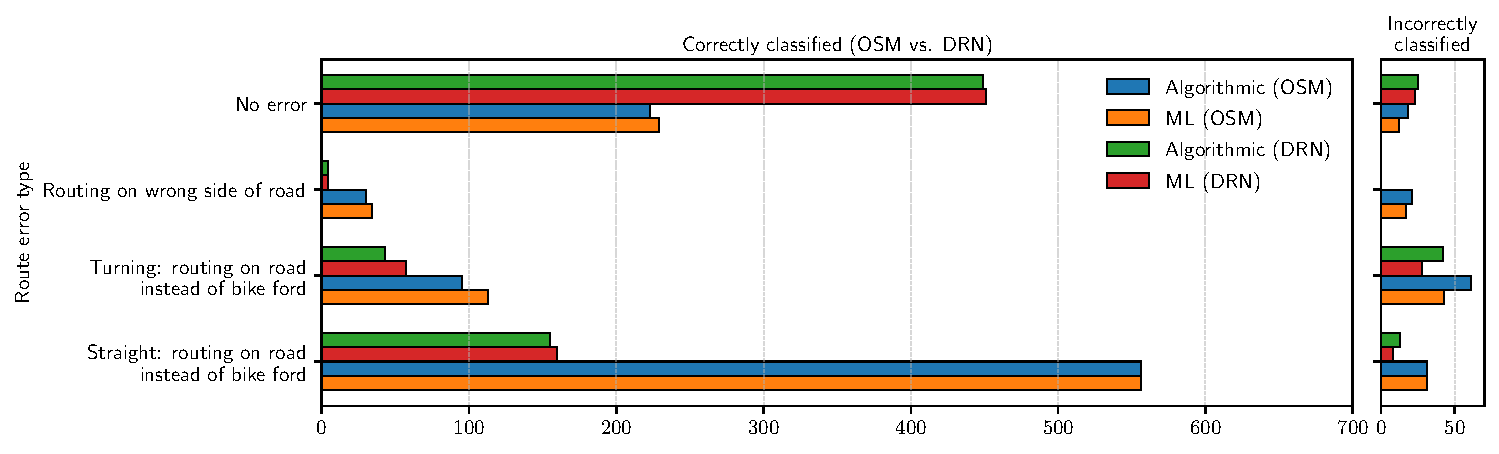
\includegraphics[width=\linewidth]{images/matching-route-errors-osm-vs-drn.pdf}
\caption{.}
\label{fig:}
\end{figure}

\subsection{Comparison with User Trajectories}

- Comparison routing with actual GPS trajectories (map-matching)

- Evaluation rerouting-points, avoided segments

\section{Conclusions}